\documentclass[11pt]{article}

% Change "review" to "final" to generate the final (sometimes called camera-ready) version.
% Change to "preprint" to generate a non-anonymous version with page numbers.
\usepackage[review]{acl}
%\usepackage[preprint]{acl}
% Standard package includes
\usepackage{times}
\usepackage{latexsym}


\usepackage{tikz}
\usetikzlibrary{arrows.meta,positioning}

\usepackage{pgfplots}
\pgfplotsset{compat=1.18}
\usepackage{booktabs}
\usepackage{multirow}
\usepackage{xcolor}
% 定义一些强调色，用于Highlight SOTA
\newcommand{\best}[1]{\textbf{\textcolor{blue!70!black}{#1}}} % SOTA
\newcommand{\better}[1]{\underline{#1}} % 超过金牌线


% Preamble (optional)
\usepackage[most]{tcolorbox}
\usepackage{booktabs}
\usepackage{enumitem}
\newcommand{\pts}[1]{\qquad{\small(#1 pts)}}
% Preamble (add if not already in your ACL file)
\usepackage{booktabs}
\usepackage{pifont}
\newcommand{\cmark}{\ding{51}}
\newcommand{\xmark}{\ding{55}}

% in preamble
\usepackage{booktabs}
\usepackage{tabularx}
\usepackage{array}

% nicer TabularX "X" column (left-aligned, allows \newline)
\newcolumntype{Y}{>{\raggedright\arraybackslash}X}

% --- Consistent two-line card header ---
\newcommand{\CardHeader}[2]{%
\begin{tabular}{@{}l@{}}
{\Large\bfseries #1}\\[-0.15em]
{\normalsize\itshape #2}
\end{tabular}
}


% For proper rendering and hyphenation of words containing Latin characters (including in bib files)
\usepackage[T1]{fontenc}
% For Vietnamese characters
% \usepackage[T5]{fontenc}
% See https://www.latex-project.org/help/documentation/encguide.pdf for other character sets

% This assumes your files are encoded as UTF8
\usepackage[utf8]{inputenc}

% This is not strictly necessary, and may be commented out,
% but it will improve the layout of the manuscript,
% and will typically save some space.
\usepackage{microtype}

% This is also not strictly necessary, and may be commented out.
% However, it will improve the aesthetics of text in
% the typewriter font.
\usepackage{inconsolata}

%Including images in your LaTeX document requires adding
%additional package(s)
\usepackage{graphicx}
\usepackage{caption} % for \captionof inside tcolorbox (no floats)

% If the title and author information does not fit in the area allocated, uncomment the following
%
%\setlength\titlebox{<dim>}
%
% and set <dim> to something 5cm or larger.

\newcommand{\medal}[1]{\raisebox{-0.25\height}{\includegraphics[height=1.15em]{#1}}}

\newcommand{\WinnerMedal}{\medal{latex/medal/trophy.png}}
\newcommand{\GoldMedal}{\medal{latex/medal/gold.png}}
\newcommand{\SilverMedal}{\medal{latex/medal/silver.png}}
\newcommand{\BronzeMedal}{\medal{latex/medal/bronze.png}}
\newcommand{\ClownMedal}{\medal{latex/medal/clown.png}}


% 在数字后面加 medal
\newcommand{\Winner}[1]{\WinnerMedal\,#1}
\newcommand{\Gold}[1]{\GoldMedal\,#1}
\newcommand{\Silver}[1]{\SilverMedal\,#1}
\newcommand{\Bronze}[1]{\BronzeMedal\,#1}
\newcommand{\Clown}[1]{\ClownMedal\,#1}


\title{Science Arena: Time-Release Olympiad Exams for Rubric-Faithful Evaluation of Scientific Reasoning}

% Author information can be set in various styles:
% For several authors from the same institution:
% \author{Author 1 \and ... \and Author n \\
%         Address line \\ ... \\ Address line}
% if the names do not fit well on one line use
%         Author 1 \\ {\bf Author 2} \\ ... \\ {\bf Author n} \\
% For authors from different institutions:
% \author{Author 1 \\ Address line \\  ... \\ Address line
%         \And  ... \And
%         Author n \\ Address line \\ ... \\ Address line}
% To start a separate ``row'' of authors use \AND, as in
% \author{Author 1 \\ Address line \\  ... \\ Address line
%         \AND
%         Author 2 \\ Address line \\ ... \\ Address line \And
%         Author 3 \\ Address line \\ ... \\ Address line}

\author{xxx \\
  \texttt{email@domain} \\\And
  xxx \\
  \texttt{email@domain} \\}

%\author{
%  \textbf{First Author\textsuperscript{1}},
%  \textbf{Second Author\textsuperscript{1,2}},
%  \textbf{Third T. Author\textsuperscript{1}},
%  \textbf{Fourth Author\textsuperscript{1}},
%\\
%  \textbf{Fifth Author\textsuperscript{1,2}},
%  \textbf{Sixth Author\textsuperscript{1}},
%  \textbf{Seventh Author\textsuperscript{1}},
%  \textbf{Eighth Author \textsuperscript{1,2,3,4}},
%\\
%  \textbf{Ninth Author\textsuperscript{1}},
%  \textbf{Tenth Author\textsuperscript{1}},
%  \textbf{Eleventh E. Author\textsuperscript{1,2,3,4,5}},
%  \textbf{Twelfth Author\textsuperscript{1}},
%\\
%  \textbf{Thirteenth Author\textsuperscript{3}},
%  \textbf{Fourteenth F. Author\textsuperscript{2,4}},
%  \textbf{Fifteenth Author\textsuperscript{1}},
%  \textbf{Sixteenth Author\textsuperscript{1}},
%\\
%  \textbf{Seventeenth S. Author\textsuperscript{4,5}},
%  \textbf{Eighteenth Author\textsuperscript{3,4}},
%  \textbf{Nineteenth N. Author\textsuperscript{2,5}},
%  \textbf{Twentieth Author\textsuperscript{1}}
%\\
%\\
%  \textsuperscript{1}Affiliation 1,
%  \textsuperscript{2}Affiliation 2,
%  \textsuperscript{3}Affiliation 3,
%  \textsuperscript{4}Affiliation 4,
%  \textsuperscript{5}Affiliation 5
%\\
%  \small{
%    \textbf{Correspondence:} \href{mailto:email@domain}{email@domain}
%  }
%}

\begin{document}
\maketitle
\begin{abstract}
Benchmark saturation and data contamination make it increasingly difficult to measure genuine scientific reasoning in frontier LLMs. We introduce \textsc{Science Arena}, an olympiad-style evaluation suite built from five rubric-driven scientific competitions whose official materials were publicly released in Aug/Oct 2025 (plus IBO 2023 released in 2025), forming a practical time-release holdout against pretraining overlap. To approximate real exam conditions, olympiad medalists grade model solutions with stepwise partial-credit rubrics, and we map scores to medal-calibrated human baselines. Across Physics, Chemistry, and Biology theory exams, the best model reaches or exceeds the Human-Gold tier; it even surpasses the Human Winner on IBO'23, which uses a more objectively scorable (constrained-format) test, but remains below Human-Winner performance on open-ended IPhO/IChO where long-form derivations and partial credit dominate. We further show LLM-as-a-judge can substantially inflate scores on open-ended chemistry, motivating expert, rubric-faithful evaluation. Finally, we provide an expert-derived cross-domain ability boundary that pinpoints remaining bottlenecks such as visual grounding and long-horizon coherence.


\end{abstract}


\section{Introduction}
Scientific reasoning has become a central target for frontier LLMs, yet evaluation is at an impasse.
Popular benchmarks are increasingly saturated and vulnerable to contamination \citep{hendrycks2021mmlu,rein2023gpqa,white2024livebench}, while “fresh” or time-sensitive constructions often remain confined to simple fill-in-the-blank or multiple-choice formats, failing to capture the multi-step derivations, partial credit nuances, and multimodal grounding essential to scientific inquiry \citep{latesteval2023,white2024livebench,wang2023scibench,yue2023mmmu,he2024olympiadbench,lu2022scienceqa,mirza2025chembench}.

A second bottleneck is \emph{measurement}.
Open-ended science evaluation is often delegated to automated judges due to cost, but LLM-based judging is known to be imperfect even in chatbot-style settings \citep{zheng2023judging}; the challenge is sharper for olympiad rubrics where “nearly-right” steps, diagram/structure fidelity, and error-forward rules determine partial credit.
As a result, automated evaluation frequently leads to score inflation, masking fragile reasoning behaviors that matter in real exams.

We present \textsc{Science Arena}, a competition-simulation benchmark derived from five high-stakes scientific competitions released in late 2025, designed as an uncontaminated holdout akin to prior work on competition-based evaluation \citep{balunovic2025matharena}.
Sec. \ref{sec:2} describes the benchmark sources, rubric-faithful expert grading, and our stateful protocol for multi-part problems.
Sec. \ref{sec:3} reports (i) medal-calibrated standings on international exams under expert grading, (ii) an ablation of iterative vs.\ one-shot protocols, (iii) a stress test of LLM-as-a-judge reliability, and (iv) an expert-derived ability boundary highlighting where frontier models still fail.

\paragraph{Contributions.}
(1) We release \textsc{Science Arena}, an olympiad-style, time-release holdout for scientific reasoning.
(2) We provide medal-calibrated, rubric-faithful expert grading that reveals failure modes hidden by automated evaluation.
(3) We offer diagnostic analyses (protocol ablation; ability boundary) to localize remaining gaps in scientific reasoning.





\section{Science Arena}\label{sec:2}
We introduce \textsc{Science Arena}, a benchmark suite built from five high-stakes science competitions with well-defined problem structure and explicit marking schemes.

\subsection{Competitions Sources}

% --- Table (requires \usepackage{booktabs,tabularx} ) ---
\begin{table}[t]
\centering
\footnotesize
\setlength{\tabcolsep}{4pt}
\renewcommand{\arraystretch}{1.08}
\begin{tabular}{l l c c c}
\toprule
\textbf{Exam} & \textbf{Release} & \textbf{International} & \textbf{Open\_ended} & \textbf{Scores} \\
\midrule
IPhO'25 & Aug 2025 & \cmark & \cmark & 30 \\
IChO'25 & Aug 2025 & \cmark & \cmark & 60 \\
IBO'23  & Aug 2025$^\dagger$ & \cmark & \xmark & 453 \\
CChO'25 & Oct 2025 & \xmark & \cmark & 100 \\
CPhO'25 & Oct 2025 & \xmark & \cmark & 320 \\
\bottomrule
\end{tabular}
\vspace{-0.3em}
\caption{\textsc{Science Arena} sources. $^\dagger$IBO papers follow a two-year blackout policy; thus IBO~2023 becomes public in 2025. }
\vspace{-0.8em}
\label{tab:science_arena_sources}
\end{table}
As in Table~\ref{tab:science_arena_sources}, we test LLMs on the latest Olympiad competitions. These are top-tier international competitions held in the second half of 2025. Consequently, they serve as an effective benchmark for evaluating prior models to ascertain their true capabilities.

% \begin{tcolorbox}[
%   title={A case of IPhO 2025 problem. (stylized vignette)},
%   colback=gray!3,
%   colframe=black!35,
%   boxrule=0.6pt,
%   arc=1.5mm,
%   left=1.5mm,right=1.5mm,top=1mm,bottom=1mm
% ]
% \small
% \textbf{Context (excerpt).}
% A problem spans multiple subparts and mixes symbolic derivation with extracting numbers from a figure.
% You may assume standard constants ($G,\hbar,e,\ldots$).

% \vspace{0.2em}
% \begin{enumerate}[leftmargin=1.2em,itemsep=0.2em]
%   \item \textbf{Derivation.} A particle moves in a central field. Derive a relation between $v(r)$ and $r$,
%         and obtain an expression for an energy scale $E(r)$. \pts{0.8}
%   \item \textbf{Read a graph.} From a given figure, read $v$ at two radii ($r_1,r_2$) and estimate
%         enclosed masses $M(<r_i)=r_i v(r_i)^2/G$. Briefly interpret whether the outer region suggests an additional component. \pts{1.0}
%   \item \textbf{Regimes / threshold.} A system changes behavior depending on a control parameter $\xi$.
%         Find a threshold $\xi^\star$ separating two regimes and state which forces/constraints set it. \pts{0.8}
%   \item \textbf{Representation.} Sketch (or describe) the required diagram (e.g., a loop/trajectory) that supports your
%         work/energy calculation, and label key points. \pts{0.4}
% \end{enumerate}
% \label{fig:example}
% \end{tcolorbox}

\begin{figure}[htbp]
    \centering
    % 这里的 tcolorbox 内容我原封不动地保留了
    \begin{tcolorbox}[
      title={A case of IPhO 2025 problem. (stylized vignette)},
      colback=gray!3,
      colframe=black!35,
      boxrule=0.6pt,
      arc=1.5mm,
      left=1.5mm,right=1.5mm,top=1mm,bottom=1mm
    ]
    \small
    \textbf{Context (excerpt).}
    A problem spans multiple subparts and mixes symbolic derivation with extracting numbers from a figure.
    You may assume standard constants ($G,\hbar,e,\ldots$).

    \vspace{0.2em}
    \begin{enumerate}[leftmargin=1.2em,itemsep=0.2em]
      \item \textbf{Derivation.} A particle moves in a central field. Derive a relation between $v(r)$ and $r$,
            and obtain an expression for an energy scale $E(r)$. \pts{0.8}
      \item \textbf{Read a graph.} From a given figure, read $v$ at two radii ($r_1,r_2$) and estimate
            enclosed masses $M(<r_i)=r_i v(r_i)^2/G$. Briefly interpret whether the outer region suggests an additional component. \pts{1.0}
      \item \textbf{Regimes / threshold.} A system changes behavior depending on a control parameter $\xi$.
            Find a threshold $\xi^\star$ separating two regimes and state which forces/constraints set it. \pts{0.8}
      \item \textbf{Representation.} Sketch (or describe) the required diagram (e.g., a loop/trajectory) that supports your
            work/energy calculation, and label key points. \pts{0.4}
    \end{enumerate}
    \end{tcolorbox}

    % 这里添加 caption 解决了“没描述”和“编号引用错误”的问题
    \caption{A representative example from IPhO 2025 illustrating diverse scientific reasoning skills.}
    
    % Label 必须放在 Caption 后面，这样引用才是 Figure X，而不是章节号
    \label{fig:example}
\end{figure}
From Figure~\ref{fig:example}, we can see a representative example from one of our competitions, IPhO 2025, illustrating that such tasks probe a diverse set of scientific reasoning skills—\emph{symbolic derivation}, \emph{quantitative graph-to-number extraction}, \emph{regime/threshold analysis}, and \emph{clear diagrammatic representation}—rather than mere factual recall. 
We analyze LLMs' abilities in Sec .~\ref {sec:llm-ability}

\subsection{Rubric-Faithful Scoring}
Leveraging the granular scoring rubrics provided in the competition, we evaluate models in a manner analogous to human exam assessment, combining \textbf{manual grading} with \textbf{automated evaluation\footnote{We use \textbf{Gemini 3 pro (preview)}  as the judge model for automated evaluation.}}. We compare them in Sec .~\ref {sec:test-eval-type}.

Our evaluators are distinguished medalists in their respective fields. We focused the human evaluation on international competitions, using a dual-expert review process to bolster result reliability. 


\subsection{Solving Protocols}

\begin{figure}[t]
\centering
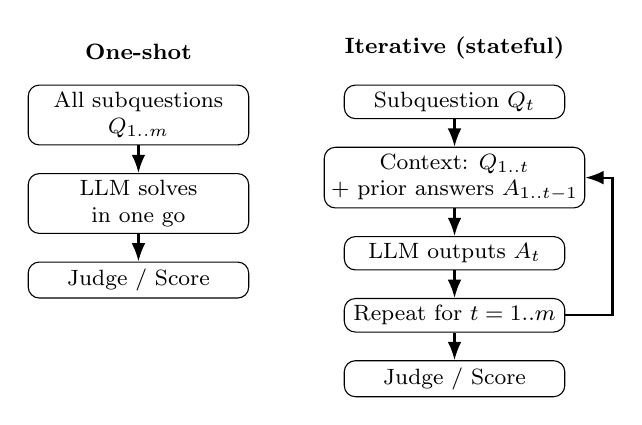
\begin{tikzpicture}[
  font=\footnotesize,
  >={Latex[length=2mm]},
  node distance=3.5mm and 10mm,
  box/.style={draw, rounded corners, align=center, inner sep=2.5pt, minimum width=28mm},
  line/.style={-Latex, thick}
]

% --- One-shot (left) ---
\node[box] (A0) {All subquestions\\$Q_{1..m}$};
\node[box, below=of A0] (A1) {LLM solves\\in one go};
\node[box, below=of A1] (A2) {Judge / Score};
\draw[line] (A0) -- (A1);
\draw[line] (A1) -- (A2);
\node[above=2mm of A0, font=\footnotesize\bfseries] {One-shot};

% --- Iterative (right) ---
\node[box, right=12mm of A0.north east, anchor=north west] (B0) {Subquestion $Q_t$};
\node[box, below=of B0] (B1) {Context: $Q_{1..t}$\\+ prior answers $A_{1..t-1}$};
\node[box, below=of B1] (B2) {LLM outputs $A_t$};
\draw[line] (B0) -- (B1);
\draw[line] (B1) -- (B2);

% loop + final scoring (compact)
\node[box, below=of B2] (B3) {Repeat for $t=1..m$};
\node[box, below=of B3] (B4) {Judge / Score};
\draw[line] (B2) -- (B3);
\draw[line] (B3) -- (B4);
\draw[line] (B3.east) -- ++(6mm,0) coordinate (loop)
            -- (loop |- B1.east) -- (B1.east);


\node[above=2mm of B0, font=\footnotesize\bfseries] {Iterative (stateful)};

\end{tikzpicture}
\caption{Two protocols for multi-part problems: one-shot solving vs. iterative, stateful prompting.}
\label{fig:one-shot-vs-iterative}
\end{figure}
Most physics and chemistry competition questions are structured as comprehensive problems with multiple sub-parts. Addressing the lack of a unified evaluation standard, we explored both joint and iterative generation methods. They are compared in Figure~\ref{fig:one-shot-vs-iterative}, which generates answers for each sub-question sequentially. We use iterative evaluation as the default. We further conduct an ablation study in Section~\ref{sec:ablation_iterative_oneshot} to systematically compare iterative prompting against the one-shot baseline.

\subsection{Models}
We categorize the evaluated LLMs into two distinct groups: those released on or before early August 2025, and those released after September 2025:
\begin{itemize}[leftmargin=*, noitemsep, topsep=2pt]
    \item \textbf{Before early August 2025}: \emph{Gemini~2.5~Pro} \citep{deepmind_gemini25pro_modelcard_2025,comanici2025gemini25}, \emph{GPT-5} \citep{openai_gpt5_systemcard_2025}, \emph{DeepSeek~V3.1} \citep{deepseekv3_1_modelcard_2025}, \emph{Qwen3~235B} \citep{yang2025qwen3,qwen3_235b_a22b_instruct_2507}, and \emph{GLM~4.5} \citep{glm45_arc_2025}.
    \item \textbf{After September 2025}: \emph{Gemini~3~Pro (preview)} \citep{deepmind_gemini3pro_modelcard_2025}, \emph{Gemini~3~Flash (preview)} \citep{deepmind_gemini3flash_modelcard_2025}, \emph{Claude~Opus~4.5} \citep{anthropic_claude45_systemcard_2025}, \emph{DeepSeek~V3.2} \citep{deepseekv3_2_technical_report_2025}, \emph{GPT-5.1} \citep{openai_gpt5_1_systemcard_addendum_2025}, and \emph{GLM~4.7} \citep{glm47_modelcard_hf_2025,glm47_techblog_2025}.
\end{itemize}

\section{Results and Diagnostics}\label{sec:3}

\subsection{Expert-Graded Results on International Competitions}
\begin{table}[t]
\centering
\small
\begin{tabular}{lrrr}
\toprule
\textbf{Metric} & \textbf{IPHO 25} & \textbf{ICHO 25} & \textbf{IBO 23} \\
% \textit{Format} & \textit{Open-ended} & \textit{Open-ended} & \textit{Multiple Choice} \\
\textit{Full Scores} & \textit{30.0} & \textit{60.0} & \textit{453.0} \\
\midrule
\multicolumn{4}{l}{\textit{\textbf{Human Benchmarks}}} \\
\quad \Winner{Human Winner} & 29.2 & 57.1 & 395.4 \\
\quad \Gold{Human Gold}  & 23.4 & 36.6 & 354.7 \\
\quad \Silver{Human Silver} & 17.0 & 28.7 & 293.1 \\
\quad \Bronze{Human Bronze} & 11.5 & 26.3 & 249.7 \\
\midrule
\multicolumn{4}{l}{\textit{\textbf{Model Performance}}} \\
\quad Gemini 2.5 Pro
  & \Gold{\best{{24.1}}}
  & \Gold{\best{{37.0}}}
  & \Winner{\best{{404.0}}} \\
\quad GPT-5
  & \Silver{21.8}
  & \Silver{31.8}
  & \Gold{{395.0}} \\
\quad GLM 4.5
  & \Silver{21.2}
  & 19.8
  & \Silver{329.0} \\
\quad DeepSeek V3.1
  & \Silver{19.4}
  & \Bronze{26.6}
  & \Silver{312.0} \\
\quad Qwen3 235B
  & \Bronze{15.2}
  & 25.9
  & \Silver{337.0} \\
\bottomrule
\end{tabular}
\caption{Results on Uncontaminated Science Olympiad Datasets (August 2025), all models listed above are released before this handoff. The best model performance is \best{bolded}. All scores are rated by experts.}
\label{tab:main_results}
\end{table}



Table~\ref{tab:main_results} reports expert-graded results on these uncontaminated exams, with all models released prior to the competitions\footnote{IPHO/ICHO/IBO include theory and practical parts; we evaluate only the theory portion.
Medal cutoffs are defined as the average theory score of contestants receiving each medal in the official final rankings (Gold/Silver/Bronze), rather than minimum-to-medal thresholds.}.
Gemini~2.5~Pro is the only model that consistently exceeds the Human-Gold baseline, yet a clear gap to Human-Winner remains on open-ended Physics and Chemistry, indicating that long-horizon scientific reasoning is still bottlenecked.






\subsection{Reliability of LLM-as-a-Judge}~\label{sec:test-eval-type}

Automated judging substantially inflates scores on IChO'25 compared to expert grading:
\emph{Gemini 2.5 Pro} increases from \textbf{37.0} (human; Table~\ref{tab:main_results})
to \textbf{45.4} (LLM-judge; Table~\ref{tab:longitudinal_results}), and \emph{GPT-5} from
\textbf{31.8} to \textbf{42.1}. The gap is notably smaller on IPhO ($\sim$1--2 points),
suggesting chemistry—especially structure questions with partial credit—creates a harder judging regime.
Figure~\ref{fig:judge_cases} highlights two common error modes: rubric mis-grounding and permissive matching.
\vspace{-0.3em}
\begin{figure}[!h]
    \centering

    \begin{tcolorbox}[
      title={Case A: \textbf{Mis-grounded rubric} $\Rightarrow$ spurious partial credit (IChO'25 Q1.3)},
      colback=gray!3,
      colframe=black!35,
      boxrule=0.6pt,
      arc=1.5mm,
      left=1.5mm,right=1.5mm,top=1mm,bottom=1mm
    ]
    \footnotesize
    \textbf{Task.} Draw the structures of compounds $E$ and $F$ (no stereochemistry required).\\
    \textbf{Candidate answer (LLM solve).} Proposes a \emph{wrong core scaffold} and argues the given molecular
    formula is a typo; propagates this scaffold into $F$.\\
    \textbf{Human grading.} $E$: 0/3,\; $F$: 0/3 (wrong ring system; not an error-forward-eligible variant).\\
    \textbf{LLM-as-judge.} Assigns \emph{non-zero} score (e.g., $E$: 1/3, $F$: 3/3) by (i) hallucinating an
    incompatible ``standard answer'' and (ii) applying an error-forward assumption on an already-invalid structure.
    \end{tcolorbox}

    \vspace{-0.7em}

    \begin{tcolorbox}[
      title={Case B: \textbf{Overly permissive} $\Rightarrow$ vague structures counted as correct (IChO'25 Q1.1)},
      colback=gray!3,
      colframe=black!35,
      boxrule=0.6pt,
      arc=1.5mm,
      left=1.5mm,right=1.5mm,top=1mm,bottom=1mm
    ]
    \footnotesize
    \textbf{Task.} Draw the structures of i-Cy, $A$, and $B$ (no stereochemistry required).\\
    \textbf{Candidate answer (LLM solve).} Provides high-level descriptions (keywords like ``bicyclic'',
    ``exocyclic methylene''), but \emph{does not clearly specify double-bond placement} and gives an
    \emph{unusable sketch} for i-Cy/$A$.\\
    \textbf{Human grading.} i-Cy: 0,\; $A$: 0,\; $B$: 2 (only $B$ is creditable via error-forward).\\
    \textbf{LLM-as-judge.} Awards \emph{near/full marks} by matching surface cues in the explanation while ignoring
    the key requirement: an unambiguous structural specification.
    \end{tcolorbox}

    \caption{Two typical failure modes of LLM-based judges on open-ended chemistry questions:
    (A) rubric/answer-key hallucination leading to unjustified partial credit; (B) permissive keyword matching that
    over-rewards under-specified structures.}
    \label{fig:judge_cases}
\end{figure}






\subsection{Temporal Evolution \& Scalability}
We extend our analysis to late-2025 benchmarks (CChO and CPhO) using purely automated LLM-based evaluation to track longitudinal evolution (Table~\ref{tab:longitudinal_results}).
Unlike the expert grading in Table~\ref{tab:main_results}, these scores are produced entirely by an LLM-as-a-judge.
Consequently, absolute scores—including those for IChO'25 and IPhO'25—are not directly comparable across tables; discrepancies in the common entries arise solely from the evaluation method rather than model differences.

Three qualitative trends emerge from the automated evaluation:
\begin{itemize}[leftmargin=*, noitemsep, topsep=2pt]
    \item \textbf{Generational Leaps:} Newer architectures show substantial gains. The Gemini~3 series achieves a $\sim$25\% improvement over the GPT-5 era on CChO, confirming that complex scientific reasoning is far from saturation.
    \item \textbf{Optimization vs.\ Scale:} Scaling is not monotonic under automated judging: the larger Gemini~3 model leads on chemistry (CChO; IChO), while the latency-optimized variant performs better on physics (CPhO; IPhO).
    \item \textbf{Uneven Domain Mastery:} A clear subject-wise divergence persists. Models approach saturation on CPhO ($\sim$94\%), yet struggle with CChO ($\sim$60\%), highlighting that long-horizon chemical reasoning still lags behind physical problem-solving.
\end{itemize}

\begin{table}[h]
\centering
\small
\setlength{\tabcolsep}{2.5pt}
\renewcommand{\arraystretch}{0.92}
\resizebox{\columnwidth}{!}{
\begin{tabular}{lcccc}
\toprule
\textbf{Benchmark (2025)} & \textbf{CCHO} & \textbf{CPHO} & \textbf{ICHO} & \textbf{IPHO} \\
\textit{Region} & \textit{China} & \textit{China} & \textit{Int'l} & \textit{Int'l} \\
\textit{Full Scores} & \textit{100} & \textit{320} & \textit{60} & \textit{30} \\
\midrule
\multicolumn{5}{l}{\textit{Reference / Early 2025}} \\
\quad Gemini 2.5 Pro & 55.1 & 273.0 & 45.4 & 25.3 \\
\quad GPT-5 & 47.1 & 270.0 & 42.1 & 23.5 \\
\quad GLM 4.5 & 35.0 & 221.0 & 27.5 & 20.1 \\
\quad DeepSeek V3.1 & 40.1 & 221.0 & 30.3 & 20.7 \\
\midrule
\multicolumn{5}{l}{\textit{Recent / Late 2025}} \\
\quad Gem 3 Flash Prev & \underline{59.4} & \textbf{301.5} & \underline{53.8} & \textbf{27.9} \\
\quad Gem 3 Pro Prev & \textbf{64.3} & {275.0} & \textbf{54.4} & \underline{27.2} \\
\quad GPT-5.1 High & 48.4 & \underline{285.0} & 41.0 & 24.6 \\
\quad Claude 4.5 Opus & 51.1 & 237.0 & 47.1 & 22.5 \\
\quad GLM 4.7 & 38.8 & 231.0 & 38.4 & 24.2 \\
\quad DeepSeek V3.2 & 42.2 & 248.0 & 36.1 & 19.3 \\
\bottomrule
\end{tabular}
}
\caption{Model performance evolution on extended benchmarks under \textbf{automated LLM-based evaluation}.
All scores in this table are produced by an LLM judge.
IChO'25 and IPhO'25 correspond to the same 2025 competition papers as in Table~\ref{tab:main_results}, \textbf{Bold}: Best; \underline{Underline}: Second.}
\label{tab:longitudinal_results}
\end{table}





\subsection{Protocol Sensitivity: Iterative vs.\ One-shot}\label{sec:ablation_iterative_oneshot}
We compare our iterative protocol against a one-shot baseline (Figure~\ref{fig:one-shot-vs-iterative}). Table~\ref{tab:ablation_protocol} reveals diverging trends ($\Delta = \text{Iterative} - \text{One-shot}$):

\begin{itemize}[leftmargin=*, noitemsep, topsep=2pt]
    \item \textbf{Decomposition Benefits Efficiency:} \textit{Gemini 3 Flash} gains massively (+74.5 on CPHO), confirming that iterative prompting effectively mitigates the limited reasoning window of smaller architectures.
    \item \textbf{Global Context Necessity:} Conversely, the stronger \textit{Gemini 3 Pro} degrades in Physics (-20.0). Complex physics tasks involve coupled variables; high-capacity models rely on the global context (available in one-shot) for consistency, which segmentation disrupts.
\end{itemize}

\begin{table}[h]
\centering
\small
\setlength{\tabcolsep}{3pt}
\renewcommand{\arraystretch}{0.95}
\resizebox{\columnwidth}{!}{
\begin{tabular}{lcccc}
\toprule
\multirow{2}{*}{\textbf{Model}} & \multicolumn{2}{c}{\textbf{CCHO (Chem)}} & \multicolumn{2}{c}{\textbf{CPHO (Phys)}} \\
 & \textit{Score} & \textit{$\Delta$} & \textit{Score} & \textit{$\Delta$} \\
\midrule
Gem 3 Flash Prev & 59.4 & \textcolor{teal}{+6.3} & 301.5 & \textcolor{teal}{\textbf{+74.5}} \\
Gem 3 Pro Prev & 64.3 & \textcolor{teal}{+6.7} & 275.0 & \textcolor{purple}{-20.0} \\
GPT-5.1 High & 48.4 & \textcolor{teal}{+1.7} & 285.0 & \textcolor{purple}{-8.0} \\
Claude 4.5 Opus & 51.1 & \textcolor{teal}{+7.2} & 237.0 & \textcolor{teal}{+7.0} \\
\bottomrule
\end{tabular}
}
\caption{Impact of the iterative protocol. \textit{Flash} relies on decomposition, while \textit{Pro} utilizes global context in Physics.}
\label{tab:ablation_protocol}
\end{table}











\subsection{Ability Boundary Across Domains}~\label{sec:llm-ability}

\begin{figure}[t]
    \centering
    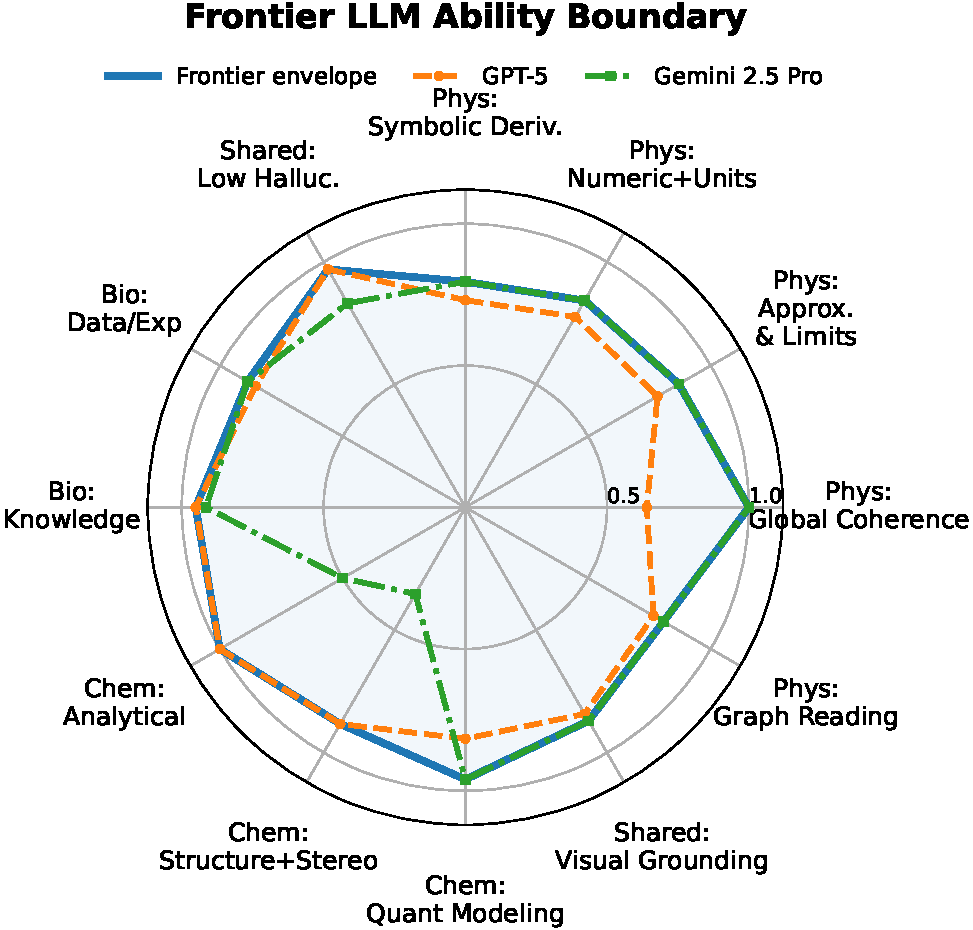
\includegraphics[width=\linewidth]{fig_llm_ability_boundary_radar_v5.2.pdf}
    \caption{\textbf{Frontier LLM ability boundary} aggregated from IPhO'25 (Physics), IChO'25 (Chemistry), and IBO'23 (Biology).
    Axes are explicitly labeled as \texttt{Phys/Chem/Bio} (domain-specific) or \texttt{Shared} to avoid ambiguity.
    The \textit{frontier envelope} reports the best value among GPT-5 and Gemini 2.5 Pro for each axis.}
    \label{fig:llm_ability_radar}
\end{figure}

Figure~\ref{fig:llm_ability_radar} summarizes a cross-domain profile beyond aggregate scores.
Frontier models are consistently strong in \textit{quantitative execution} (Physics derivation, units, approximations; Chemistry quantitative modeling)
and in \textit{biology knowledge} under constrained answer formats.
In contrast, the sharpest remaining boundary is \textit{faithful grounding}: binding non-text evidence to precise symbolic commitments
(\texttt{Shared: Visual Grounding}) and maintaining calibration (\texttt{Shared: Low Halluc.}).

To make the visualization interpretable and reproducible, we provide (i) an axis glossary (Appendix, Ability Axis Glossary) and
(ii) per-domain radars using domain-native decompositions (Appendix Figure~\ref{fig:radar_ipho25}--\ref{fig:radar_ibo23}).



\section{Conclusion}
\textsc{Science Arena} evaluates frontier LLMs under an olympiad-style, uncontaminated time-release holdout with rubric-faithful expert grading.
While the best model attains Human-Gold tier on multiple theory exams, a persistent gap to Human-Winner performance remains.
Our diagnostics identify visual grounding and global coherence as dominant bottlenecks, and we find automated judging can overestimate performance on open-ended chemistry, reinforcing the need for expert, rubric-driven evaluation.


\section*{Limitations}
Our benchmark is limited in scale and covers only five competitions; results may not generalize to all scientific curricula.
We evaluate theory components only, since experimental sections require physical apparatus and proctoring.
Expert grading is costly and thus applied primarily to international exams; some extended results rely on automated judging and should be interpreted qualitatively.
Finally, our ability taxonomy is expert-derived and may reflect annotator priors; alternative decompositions could yield different boundary shapes.

% \section*{Acknowledgments}

\bibliography{custom}

\appendix
\section{Competition Sources}
\label{app:competitions}

Science Arena is built from five Olympiad-style scientific competitions spanning physics, chemistry, and biology. A key design choice is to index each dataset by the \emph{public release time} of the official problem materials (rather than the contest year), so that evaluation can be conducted on a practical ``time-release holdout'' that reduces the likelihood of overlap with prior training corpora. Table~\ref{tab:science_arena_sources} summarizes the sources we cite for each competition.

\paragraph{International Physics Olympiad (IPhO 2025).}
We use the official IPhO 2025 repository of exam materials, including the released problems and accompanying official documents (e.g., solutions and/or marking guidance when provided) \citep{ipho2025_official_questions}. IPhO exams consist of theory and experimental components; our benchmark focuses on the \emph{theory} problems, since experimental tasks require physical apparatus and proctoring conditions that are not directly reproducible for LLM evaluation.

\paragraph{International Chemistry Olympiad (IChO 2025).}
We source IChO 2025 materials from the official ``Problems'' page released by the competition organizers \citep{icho2025_problems_page}. Similar to IPhO, IChO includes theory and laboratory components; we evaluate models on the \emph{theory} portion to ensure a well-defined, reproducible setting with rubric-faithful scoring.

\paragraph{International Biology Olympiad (IBO 2023).}
IBO provides an official archive of examination papers for past competitions \citep{ibo_papers_archive}. In Science Arena, IBO 2023 serves as an \emph{objectively scorable} biology track (e.g., multiple-choice or otherwise unambiguously keyed questions), enabling automatic evaluation without judge-model mediation. When reporting medal-calibrated comparisons, we reference the official IBO 2023 results report \citep{ibo2023_final_results}.

\paragraph{China Chemistry Olympiad (CChO 2025).}
For CChO 2025, we use publicly released final-round materials (problem statements and marking guidance) distributed as a consolidated PDF \citep{ccho2025_final_theory_paper_public_pdf}. When normalizing scores and aligning evaluation to official scoring practice, we additionally cite the Chinese Chemical Society document describing the theory score conversion weights \citep{ccho2025_theory_weighting_chemsoc}. As with other laboratory-inclusive competitions, our primary benchmark setting targets the theory component for reproducibility.

\paragraph{China Physics Olympiad (CPhO 2025).}
For CPhO 2025, we use publicly released final-round theory materials and the associated marking scheme \citep{cpho2025_final_theory_paper_public_pdf,cpho2025_final_theory_solution_marking_public_pdf}. Where relevant to describing the competition formally (e.g., structure, governance, or official rules), we also cite the published competition charter \citep{cpho_charter_2025_revision}. We evaluate the theory component as the reproducible portion of the exam; experimental components and their marking documents can be referenced separately when needed \citep{cpho2025_final_practical_paper_public_pdf,cpho2025_final_practical_answer_key_public_pdf}.

\paragraph{Notes on scope and reproducibility.}
All five competitions are high-stakes, rubric-driven assessments with well-defined problem sets and (for open-ended tasks) partial-credit grading. Science Arena prioritizes the \emph{publicly released} versions of these materials to support reproducibility and transparent sourcing, and it uses theory-only evaluation where experimental replication would otherwise confound model comparisons.



\section{Details of Ability Boundary}
\label{sec:append-ability}
\subsection*{Ability Axis Glossary}
\begin{itemize}[leftmargin=*, noitemsep, topsep=2pt]
\item \textbf{Phys: Symbolic Deriv.} --- multi-step algebraic manipulation and equation-based reasoning.
\item \textbf{Phys: Numeric+Units} --- numerical accuracy with unit/scale discipline (dimensional checks, sanity bounds).
\item \textbf{Phys: Approx.\ \& Limits} --- correct approximations and limiting-case validation.
\item \textbf{Phys: Global Coherence} --- maintain consistent assumptions/variables across coupled subparts (regime tracking).
\item \textbf{Phys: Graph Reading} --- extract trends/values from curves and use them downstream.
\item \textbf{Shared: Visual Grounding} --- bind non-text evidence to symbols/claims (diagrams/structures/figures; ``read-the-figure'' reliability).
\item \textbf{Chem: Quant Modeling} --- quantitative physical chemistry (equilibria/thermo/electro) under algebraic constraints.
\item \textbf{Chem: Structure+Stereo} --- structure fidelity and stereochemical correctness (connectivity, configuration).
\item \textbf{Chem: Analytical} --- interpret analytical evidence (e.g., spectroscopy/assays) into chemically valid conclusions.
\item \textbf{Bio: Knowledge} --- biology knowledge and reading comprehension in constrained formats (mechanisms/terminology).
\item \textbf{Bio: Data/Exp} --- reasoning from experimental data (figures/tables, controls, statistical cues, causality).
\item \textbf{Shared: Low Halluc.} --- calibration/faithfulness proxy: lower rate of confidently-wrong outputs when confidence is available.
\end{itemize}
\subsection{Domain-specific ability profiles (radar plots)}
\label{app:domain_radars}

Figure~\ref{fig:radar_ipho25}--\ref{fig:radar_ibo23} summarize within-domain ability profiles.
Each radar overlays a \emph{frontier envelope} (per-axis best among the compared frontier models), GPT-5, and Gemini 2.5 Pro.
Axes are domain-native (Physics/Chemistry/Biology) and therefore are \emph{not} directly comparable across figures.

\begin{figure}[t]
  \centering
  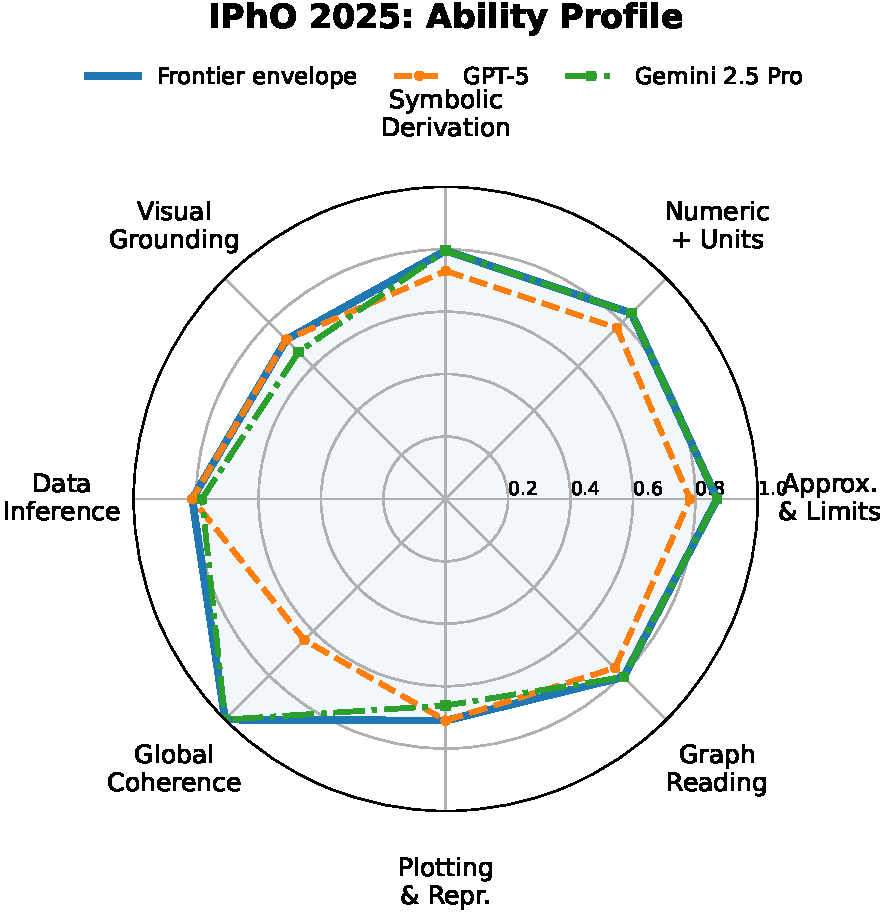
\includegraphics[width=\linewidth]{appendix_ipho2025_radar_v3.pdf}
  \caption{\textbf{IPhO 2025.} Physics abilities follow our rubric: symbolic derivation, numerical computation with units, approximation/limiting cases, graph reading, plotting/representation, global coherence across regimes, data inference from empirical relations, and visual grounding.}
  \label{fig:radar_ipho25}
\end{figure}

\noindent\textbf{IPhO 25 notes.} Both models are strongest on local symbolic manipulation and routine numerics; remaining errors concentrate in \emph{global coherence} (propagating assumptions consistently across long solutions) and \emph{visual grounding} (extracting non-textual cues), with noticeable variance across tasks requiring regime switching.

\begin{figure}[t]
  \centering
  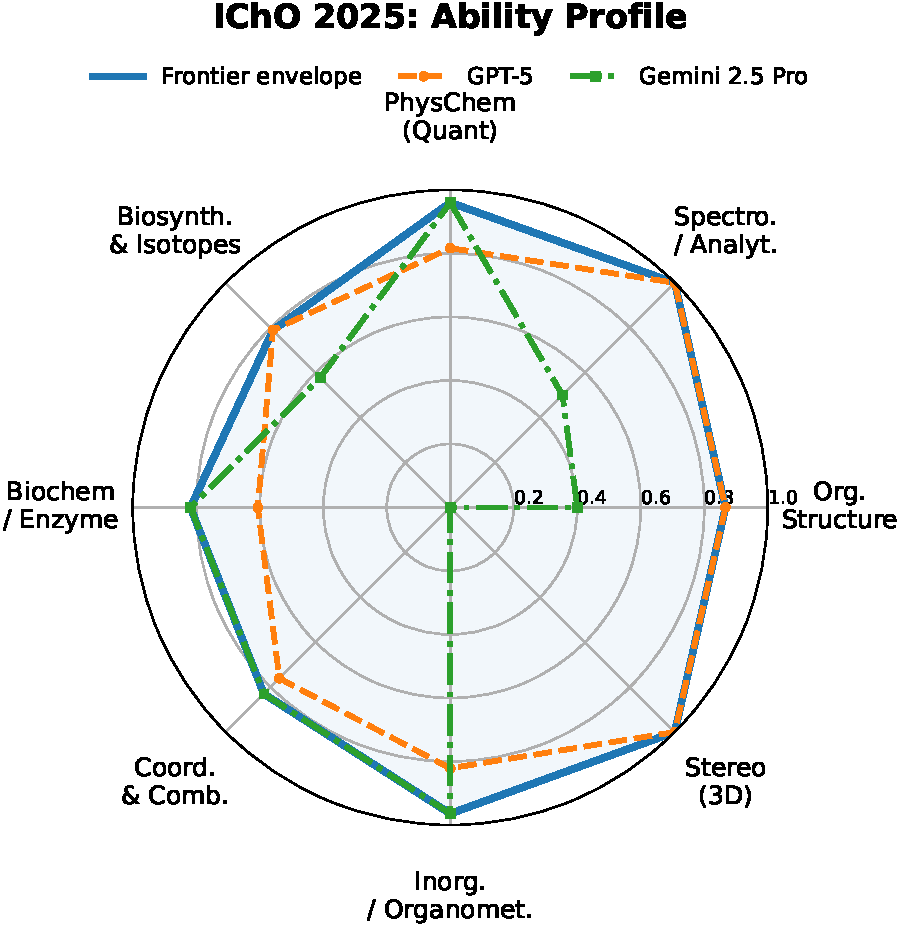
\includegraphics[width=\linewidth]{appendix_icho2025_radar_v3.pdf}
  \caption{\textbf{IChO 2025.} Chemistry abilities use the human-coded decomposition: quantitative physical chemistry; spectroscopy/analytical reasoning; organic structure depiction; stereochemistry; inorganic/organometallic reasoning; coordination/combinatorics; biochemistry/enzyme reasoning; and biosynthesis/isotopic tracing.}
  \label{fig:radar_icho25}
\end{figure}

\noindent\textbf{IChO 25 notes.} Gemini 2.5 Pro tends to be more uniformly strong on quantitative and analytical axes (physical chemistry and spectroscopy), while GPT-5 exhibits higher dispersion: it can solve isolated substeps but is less consistent when multiple constraints (structure + stereochemistry + quantitative checks) must be satisfied simultaneously.

\begin{figure}[t]
  \centering
  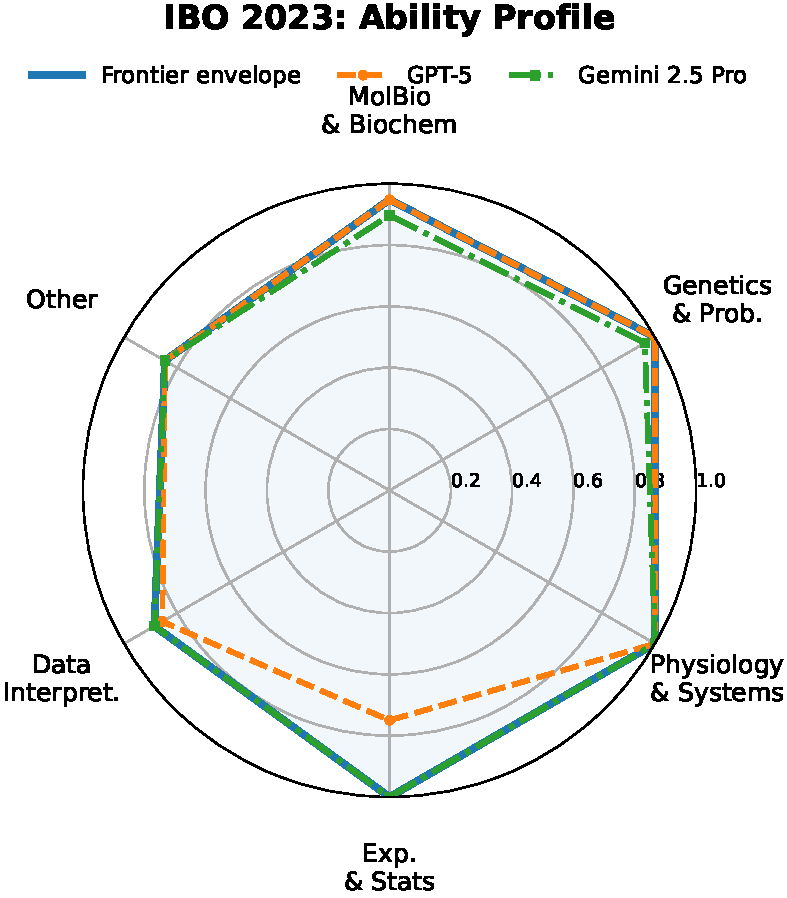
\includegraphics[width=\linewidth]{appendix_ibo2023_radar_v3.pdf}
  \caption{\textbf{IBO 2023.} Biology abilities are summarized into observed question categories derived from model outputs: molecular biology/biochemistry, genetics/probability, physiology/systems, experimental design/statistics, data/figure interpretation, and a residual ``other'' bucket.}
  \label{fig:radar_ibo23}
\end{figure}

\noindent\textbf{IBO 23 notes.} Frontier models reach near-ceiling performance on knowledge-centric multiple-choice biology (molecular biology and genetics), but are noticeably weaker on evidence-centric reasoning (statistics/design and data/figure interpretation), consistent with broader multimodal grounding limitations.


% \input{appendix_llm_ability_axis_desc_v3.tex}

% \section{Example Appendix}
% \label{sec:appendix}

% This is an appendix.

\end{document}
